\documentclass[11pt]{article}
\usepackage[letterpaper,margin=1in]{geometry}
\usepackage{xcolor}
\usepackage{fancyhdr}
% \usepackage{tgschola} % or any other font package you like
\usepackage{lastpage}
\usepackage{parskip} % Remove paragraph indentation
\usepackage{amsmath} % for align
\usepackage{amsthm} % for proof pkg
\usepackage{amssymb}
%\usepackage{tikz}
\usepackage{graphicx}
\usepackage{proof}
\usepackage{enumitem}
% \usepackage[shortlabels]{enumerate}
\usepackage{algorithm}
\usepackage{algorithmicx}
\usepackage{algpseudocode}
\usepackage{hyperref}


\newtheorem{theorem}{Theorem}[section]
\newtheorem{corollary}{Corollary}[theorem]
\newtheorem{lemma}[theorem]{Lemma}
\newtheorem{proposition}{Proposition}[section]

\renewcommand{\algorithmicrequire}{\textbf{Input:}}  % Use Input in the format of Algorithm
\renewcommand{\algorithmicensure}{\textbf{Output:}} % Use Output in the format of Algorithm  



\newcommand{\yourtitle}{CS 6220: Data-Sparse Matrix Computations}
\newcommand{\yoursubtitle}{Project Report: Global vs. Local Graph Clustering}
\newcommand{\yourname}{ajh326, aak228}


\newtheorem{claim}{Claim}

\pagestyle{fancy}
\headheight 13.6pt
\fancyhf{}
\fancyhead[L]{%
  \footnotesize%\sffamily
  \yourtitle\\
  \yoursubtitle}
\fancyhead[R]{\yourname}
\fancyfoot[C]{\thepage\ of \pageref{LastPage}}
% \usepackage[
%   colorlinks,
%   breaklinks,
%   pdftitle={\yourname - \soptitle},
%   pdfauthor={\yourname},
%   unicode
% ]{hyperref}

\begin{document}

\newcommand{\Half}{\frac{1}{2}}



\begin{center}\LARGE \yoursubtitle\\
\large Andrew Horning (ajh326), Ariah Klages-Mundt (aak228)
\end{center}

%%%%%%%%%%%%%%%%%%%%%%%%%%%%%%%%%%%%%%%%%%%%%
\section{Introduction}

Graph clustering, the partitioning of a graph into sets of `similar' nodes, has risen to prominence over the last several decades as the availability of large data sets in consumer and social networks has increased. It has become an invaluable tool for identifying communities in social networks, uncovering structure in high-dimensional data sets, and developing sophisticated recommendation systems \cite{social_network, high_dim_data, recommenders}. One particular notion of `similar' nodes is to partition graph vertices into sets of low conductance, defined below. Intuitively, one can think of the conductance of a set $S$ as the probability of transitioning from a random node in $S$ to a node outside $S$. Lower conductance therefore represents a tighter community within the graph and may serve as a measure of quality for clustered communities. Unfortunately, choosing partitions of a graph $G$ which minimize the conductance of the clusters is NP-hard, but there are approximation algorithms with theoretical guarantees. We present two such approximation ideas in this report.

Spectral graph clustering is a global method that uses the eigenvectors and eigenvalues of the graph Laplacian to identify groups of nodes that are, in some sense, well connected. There are several ways to use the spectral information of the Laplacian to accomplish this task. For instance, the eigenvector associated with the smallest nonzero eigenvalue of a connected graph's Laplacian defines a near-optimal low conductance cut. This leads to an iterative procedure that partitions the graph into multiple clusters, and theoretical recovery guarantees based on conductance between clusters can be derived. 

Alternatively, one can use a subset of the eigenvectors of the Laplacian corresponding to the smallest eigenvalues to embed the graph in a Euclidean space, after which standard distance-based clustering techniques such as $k$-means may be employed. This approach to spectral clustering has interesting connections to optimization programs such as \texttt{mincut}, \texttt{ratiocut}, and \texttt{ncut}, depending on which normalization convention is chosen for the Laplacian, that select clusters that minimize an appropriate notion of inter-cluster connectivity.

The eigenvector embedding also has connections to random walks on graphs. For instance, the distance between nodes in an eigenvector embedding is closely related to the expected commute time between the two nodes. In Section~\ref{Global spectral clustering} we will focus on the eigenvector embedding strategy, particularly on the algorithm due to Shi and Malik \cite{shi}.

For very large graphs, such as those occurring in web-browsing and social network applications, directly computing with the Laplacian can become prohibitively expensive. Rather than compute eigenvectors of the Laplacian, local clustering methods seek to recover well-connected communities in a graph by exploring local structure.

In Section~\ref{Local PageRank clustering}, we will explore the local method developed in \cite{pagerank_cluster} that uses approximate personalized PageRank vectors to find clusters of low conductance. The aim here is to get eigenvector-like information using local walks on the graph. As we noted above, the eigenvector embedding describes expected commute times between nodes. This connection motivates us to approximate eigenvector information using locally biased random walks to explore local graph structure.

The goal of a local method is to run in time better than global methods, especially given sparse graphs. Approximate Personalized PageRank (APPR) does this by spreading mass from a seed set to identify clusters with theoretical guarantees. The methods in this case focus on ways to avoid having to do matrix operations as opposed to directly formulating fast sparse linear algebra computations.

\subsection*{Notation}

Throughout this report, we use the following notational conventions. An unweighted graph with node set $V$ and edge set $E$ is denoted $G=(V,E)$. The degree of a node $v\in V$ is written $d(v)$. The adjacency matrix and degree matrix are $A$ and $D$, respectively. The complement of a subset of vertices $S$ in $V$ is denoted $S^C$. We will also use the concepts of cut, conductance, and volume throughout. The cut, volume, and conductance of a subset of nodes $S\in V$ are defined as
$$\text{cut}(S) = \# \text{ edge endpoints leaving } S = \sum_{e_{ij}\in E, v_i\in S, v_j\in S^C} 1,$$
$$\text{vol}(S) = \# \text{ edge endpoints in } S = \sum_{u\in S} d(u).$$
$$\Phi(S) = \frac{\text{cut}(S)}{\min \Big( \text{vol}(S), \text{vol}(V \setminus S) \Big)}.$$

\subsection*{Outline}

The report is organized as follows. In Section \ref{Global spectral clustering}, we discuss the eigenvector embedding strategy and our implementation of a spectral clustering algorithm. In Section \ref{Local PageRank clustering}, we survey and implement a local method based on the methods in \cite{pagerank_cluster,spielman}. In Sections \ref{Computational results} and \ref{Applications}, we analyze the performance of our implementations on the generative planted partition model and demonstrate their use in a real-world application: community detection in a social network. We conclude in Section \ref{Discussion} with a few observations on the performance and implementation of the global and local methods.


%%%%%%%%%%%%%%%%%%%%%%%%%%%%%%%%%%%%%%%%%%%%%
\section{Global spectral clustering}
\label{Global spectral clustering}

\subsection*{Eigenvector Embedding}

To motivate the eigenvector embedding, consider the problem of partitioning the vertices of a graph $G=(V,E)$ into two clusters, $C\subset V$ and its compliment $C^C \subset V$, such that the conductance $\Phi(C)$ is a minimum over all such partitions. Formally, we would like to solve the \texttt{ncut} (normalized cut) program,
\begin{equation}\label{Ncut}
 C = \text{min}_{M}\hspace{.1mm}\Phi(M).
\end{equation}

Before we begin, it is helpful to supply an overview of the connection between {\tt ncut} and the eigenvectors of the graph Laplacian. As we will see below, the minimization problem can be rephrased as a constrained minimization of the Rayleigh Quotient of the Laplacian $L=D-A$. The minimization of the Rayleigh Quotient is over structured indicator vectors which store the partition information in $M$. The indicator constraint makes the minimization problem NP-hard, so it is natural to consider relaxing this to minimize over a true subspace of real valued vectors with dimension $n$. This leads to a classical minimization problem in linear algebra, the minimization of the Rayleigh quotient, whose solution is provided by certain eigenvectors of $L$. 

Recall that the Laplacian has quadratic form $u^TLu = \sum_{i,j=1}^n a_{ij}(u_i-u_j)^2$, where $u^T$ denotes the transpose of $u$.  Here, $L\in\mathbb{R}^{n\times n}$, $u\in\mathbb{R}^n$, and $a_{ij}$ are the entries of the adjacency matrix $A$. To rewrite (\ref{Ncut}) define a characteristic vector $f$ componentwise by
\begin{equation}\label{fConstraint}
f_i = \begin{cases}
\sqrt{\frac{vol(M^C)}{vol(M)}} & i\in M, \\
-\sqrt{\frac{vol(M)}{vol(M^C)}} & i\in M^C.
\end{cases}
\end{equation}
The characteristic vector $f$ encodes the partition information into a vector. We wish to solve (\ref{Ncut}) by determining an $f$ that minimizes the conductance of $M$. The key observations in this reformulation are that the conductance $\Phi(M)$ is proportional to $f^TLf$ and that $f$ is $D$-orthonormal to the first eigenvector of the Laplacian, the vector of ones $\mathbf{1}=(1,\cdots, 1)^T$. These are the results of a few simple calculations. We find that
$$f^TLf = 2\text{vol}(V)\Phi(M),\hspace{3mm}
(Df)^T\mathbf{1} = 0, \text{ and } f^TDf =\text{vol}(V).$$

We can now write down the objective and constraints in terms of $f$ and the Laplacian $L$, as
\begin{equation}\label{Rayleigh-Ritz Problem}
\begin{gathered}
\text{min}_M f^TLf, \\
\text{s.t.}\hspace{1mm} f \hspace{1mm}\text{as in } (\ref{fConstraint}), \text{ with}\\
(Df)^T\mathbf{1}=0, f^TDf = \text{vol}(V).
\end{gathered}
\end{equation}


Since the smallest eigenvalue of the Laplacian is always zero and the corresponding eigenvector is $\mathbf{1}$, this optimization problem now looks strikingly similar to the minimization of the Rayleigh quotient for the generalized eigenvalue problem $Lx=\lambda Dx$, however, the constraint on the entries of $f$ make this problem NP-hard \cite{luxburg}. The strategy is to relax the constraint on $f$ so that its entries are real valued, in which case (\ref{Rayleigh-Ritz Problem}) is minimized by the eigenvector $x$ of $D^{-1}L$ corresponding to the second smallest eigenvalue (assuming $G$ is connected, $D$ is invertible and the generalized eigenvalue problem $Lx=\lambda Dx$ is equivalent to $D^{-1}Lx=\lambda x$).

Previously, the $j^{th}$ vertex was in the cluster $M$ if the sign of the $j^{th}$ entry of $f$ was positive, and in the cluster $M^C$ if the sign was negative. To recover the partition information, we can reassign nodes to clusters based on the entries in $v$. Alternatively, a more sophisticated scheme can be used to group the entries of $v$ into groups. Here, methods such as $k$-means may be more robust and can be used when partitioning $V$ into more than two clusters.

To partition into $k>2$ clusters, a similar analysis may be carried out. The objective function is modified so that (\ref{Ncut}) is replaced by
\begin{equation}\label{Ncut k>2}
(C_1,\cdots, C_k) = \text{min}_{(M_1,\cdots, M_k)}\sum_{i=1}^k\hspace{.1mm}\Phi(M_i).
\end{equation}
The $j^{th}$ cluster now has an indicator vector defined by
\begin{equation}\label{fConstraint2}
h_{i,j} = \begin{cases}
\sqrt{\frac{1}{vol(M_i)}} & i\in M_j \\
0 & \text{otherwise},
\end{cases}.
\end{equation}
If we denote $H$ to be the matrix with entries $h_{ij}= h_{i,j}$, then the minimization problem (\ref{Ncut k>2}) is equivalent to minimizing trace$(H'LH)$ subject to $H^TDH=I$, over $H$ as in (\ref{fConstraint2}). If this last constraint on $H$ is relaxed so that the entries of $H$ are real valued, we obtain a classical trace minimization problem. The solution is given by the matrix $X\in\mathbb{R}^{n\times k}$ whose columns are the $k$ eigenvectors of the generalized eigenvalue problem $LX=\Lambda DX$ that correspond to the $k$ smallest eigenvalues after the first zero eigenvalue.

A working algorithm for spectral clustering, which seeks to approximately minimize conductance between clusters, is therefore suggested.

\begin{algorithm}[H]
\algorithmicrequire  \hspace{2mm}Graph $G$, number of clusters $k$.
\begin{algorithmic}
	\State Compute degree matrix $D\in\mathbb{R}^{n\times n}$ and graph Laplacian $L\in\mathbb{R}^{n\times n}$ associated with graph $G$.
	\State Compute first $k+1$ eigenvectors, $x_0,\cdots, x_k$ of generalized eigenvalue problem $Lx=\lambda Dx$.
	\State Form matrix $X\in\mathbb{R}^{n\times k}$ whose $i^{th}$ column is $x_i$, $1\leq i\leq k$, and let $y_j\in\mathbb{R}^k$ be the $j^{th}$ row of $X$.
    \State Use the $k$-means algorithm to partition the points $\{y_j\}_{j=1}^n$ in $\mathbb{R}^k$ into clusters $P_1,\cdots, P_k$.
\end{algorithmic}
\algorithmicensure\hspace{2mm}$\hat C_j=\{v_i \in V: y_i\in P_j\}$, for $j=1,\cdots k$.
\caption{${\tt spec\_clust}(G,k)$} \label{alg:spec_clust}
\end{algorithm}

Because of the relaxation of the constraint on the characteristic vectors, the clusters recovered by partitioning the vertices in the eigenvector embedding are not guaranteed to be minimizers of the objective function in (\ref{Ncut k>2}). In particular, there are no guarantees that the conductance of these clusters are close to the conductance of true minimizers. However, the eigenvector problem may be solved with standard tools of linear algebra and the clustering is often observed to work quite well in practice. The distance between nodes in the eigenvector embedding also has connections to other notions of connectivity in a graph, which make the relaxation and re-assign strategy a reasonable approach. In particular, the distance between vertices $v_i$ and $v_j$ in the eigenvector embedding described above is equivalent to the expected commute time between $v_i$ and $v_j$ of a random walk on $G$. Hence, one intuitive interpretation of clusters returned by Algorithm \ref{alg:spec_clust} is that a random walk or diffusion process beginning in any one of these clusters will tend to stay within the cluster for long periods of time relative to the frequency of jumps between clusters.

Finally, different normalization conventions for the Laplacian lead to similar connections with other optimization programs such as \texttt{ratiocut} and \texttt{mincut}, which involve modifying the objective function in (\ref{Ncut})

\subsection*{Implementation}

In practice, we implement an equivalent modification of Algorithm \ref{alg:spec_clust}. Rather than solve the generalized eigenvalue problem $Lx=\lambda Dx$, we compute the eigenvectors $\hat v_1,\cdots, \hat v_k$ of the symmetric normalized Laplacian $L_s = D^{-1/2}LD^{-1/2}$. The eigenvectors $v_1,\cdots,v_k$ of $D^{-1}L$ are then obtained by the scaling $v_i=D^{-1/2}\hat v_i$ for each $1\leq i\leq k$.

To compute the eigenvectors of $L_s$, we use the sparse hermitian eigensolver {\tt eigsh} which is available in {\tt scipy.sparse.linalg}. This eigensolver utilizes the implicitly restarted Lanczos method (IRLM) provided by {\tt ARPACK}, which may be interpreted as iterative applications of a truncated, implicitly shifted QR algorithm on the tridiagonal matrix returned by the Lanczos factorization that we discussed in class. The dominant cost within each iteration is a matrix-vector product, hence, we expect the complexity to scale approximately as $O(n^2)$ for dense matrices. For Laplacians stored in sparse format with a small number of non-zeros, we expect the complexity to scale approximately as $O(n)$. 


\subsection*{Alternative spectral clustering}

As noted in the introduction, there is a version of spectral clustering that uses `sweeps' over the eigenvector corresponding to the second smallest eigenvalue to find low conductance cuts with theoretical guarantees \cite{spielman_clustering_works}. This leads to an iterative procedure to partition the graph into multiple clusters. This spectral clustering method comes with guarantees on the conductance of recovered clusters and is closely related to the Local PageRank clustering algorithm which is presented in Section~\ref{Local PageRank clustering}.

%%%%%%%%%%%%%%%%%%%%%%%%%%%%%%%%%%%%%%%%%%%%%
\section{Local PageRank clustering}
\label{Local PageRank clustering}

This section surveys the exposition in \cite{pagerank_cluster}, which describes the Approximate Personalized PageRank (APPR) algorithm for clustering graphs. APPR improves on a prior Nibble method (see \cite{spielman}) that used a sequence of random walk vectors. A PageRank vector can be described recursively, so APPR can consider a single PageRank vector in place of a sequence of random walk vectors while retaining theoretical guarantees.

Personalized PageRank is defined as the unique solution to
$$\text{pr}(\alpha,s) = \alpha s + (1-\alpha) \text{pr}(\alpha,s)W,$$
where $\alpha\in(0,1]$ is a teleportation constant, $s$ is an initial concentrated distribution over the nodes (in our case, concentrated on a single node), and $W = \frac{1}{2}(I + D^{-1}A)$ is the lazy random walk transition matrix. Note that distribution vectors are written as row vectors and so multiplied to the left of $W$. The personalized PageRank describes the distribution on the nodes from a lazy random walk on the graph where, at each step, we are transported back to the starting node $s$ with probability $\alpha$. This biases the walk so that we explore local structure without going too far in the graph. Notice that the global PageRank measure can be described as above with $s$ the uniform distribution on the nodes.

For any $\alpha$, the PageRank vector can be represented as a linear transformation of $s$: $\text{pr}(\alpha,s) = s R_\alpha$, where
$$R_\alpha = \alpha \sum_{t=0}^\infty (1-\alpha)^t W^t.$$
This means that a PageRank vector is a weighted average of lazy random walk vectors:
$$\text{pr}(\alpha,s) = \alpha \sum_{t=0}^\infty (1-\alpha)^t (sW^t).$$


\subsection*{Computing approximate PageRank}
An approximate PageRank vector $\text{apr}(\alpha,s,r)$ is defined in terms of a non-negative residual vector $r$ that satisfies
$$\text{apr}(\alpha,s,r) + \text{pr}(\alpha,r) = \text{pr}(\alpha,s).$$

The following proposition, which is similar but distinct from the definition of PageRank, allows an iterative algorithm to compute approximate PageRank vectors.

\begin{proposition} \label{prop:push}
$$\text{pr}(\alpha,s) = \alpha s + (1-\alpha) \text{pr}(\alpha,sW).$$
\end{proposition}

\begin{proof}
The linear transformation $R_\alpha$ can be written recursively
$$\begin{aligned}
R_\alpha &= \alpha \sum_{t=0}^\infty (1-\alpha)^t W^t \\
	&= \alpha I + (1-\alpha) W R_\alpha.
\end{aligned}$$
We see the result by applying $R_\alpha$ to the starting distribution $s$:
$$\begin{aligned}
\text{pr}(\alpha,s) &= sR_\alpha \\
	&= \alpha s + (1-\alpha) s W R_\alpha \\
	&= \alpha s + (1-\alpha) \text{pr}(\alpha, sW).
\end{aligned}$$
\end{proof}

We construct an algorithm for computing approximate PageRank by step-wise `pushing' mass from a residual vector $r$ to the associated approximate PageRank vector $p$. Initially, we set $p = 0$ and put all mass in $r$ on the starting node--i.e., $r=\chi_v$ where
$$\chi_v(u) = \begin{cases} 1 & \text{ if } u = v \\ 0 & \text{ otherwise}\end{cases}.$$
We then apply a number of push operations based on Prop.~\ref{prop:push} to spread mass from a single node $u$. We move $\alpha$ fraction of $r(u)$ to $p(u)$, representing the teleportation move, and spread the remaining $(1-\alpha)$ share within $r$ based on single step transitions of the lazy random walk from $u$. Throughout each push, $p$ maintains the approximate PageRank equation $P + \text{pr}(\alpha,r) = \text{pr}(\alpha,s)$. This `push' subroutine is described formally in Algorithm~\ref{alg:push}.

\begin{algorithm}[H]
\algorithmicrequire graph $G$, node $u$, approximate PageRank $p$, corresponding residual $r$
\begin{algorithmic}
	\State Let $p'=p$, $r'=r$, then make the following changes
	\State $p'(u) = p(u) + \alpha r(u)$
	\State $r'(u) = (1-\alpha)r(u)/2$
	\For {$v$ s.t. $(u,v) \in E$}
		\State $r'(v) = r(v) + (1-\alpha)r(u)/(2d(u))$
	\EndFor
\end{algorithmic}
\algorithmicensure updated PageRank $p'$ and corresponding residual $r'$
\caption{${\tt push}_u(G,p,r)$} \label{alg:push}
\end{algorithm}

After running many pushes, the residual $r$ (or, more specifically, the degree-normalized version of $r$) becomes small, making $p$ a good approximation of the PageRank vector. This is formalized in Algorithm~\ref{alg:appr}. Prop.~\ref{prop:appr_iterations} bounds the number of pushes required.

\begin{algorithm}[H]
\algorithmicrequire graph $G$, starting node $v$, $\alpha \in (0,1]$, $\varepsilon$
\begin{algorithmic}
	\State Let $p = 0$, $r = \chi_v$
	\While {$\max_{u \in V} \frac{r(u)}{d(u)} \geq \varepsilon$}
		\State Choose any vertex $u$ where $\frac{r(u)}{d(u)} \geq \varepsilon$
		\State $p,r = {\tt push}_u(G,p,r)$
	\EndWhile
\end{algorithmic}
\algorithmicensure $p = \text{apr}(\alpha,\chi_v,r)$ with $\max_{u\in V} \frac{r(u)}{d(u)} < \varepsilon$
\caption{${\tt ApproximatePageRank}(G,v,\alpha,\varepsilon)$} \label{alg:appr}
\end{algorithm}

\begin{proposition} \label{prop:appr_iterations}
Let $T$ be the total number of push operations performed by {\tt ApproximatePageRank} and let $d_i$ be the degree of the vertex used in the $i$th push. Then $\sum_{i=1}^T d_i \leq \frac{1}{\varepsilon \alpha}$.
\end{proposition}

\begin{proof}
Note that the amount of probability on the vertex pushed at time $i$ is at least $\varepsilon d_i$. Then $|r|_1$ decreases by at least $\alpha \varepsilon d_i$ over the $i$th push. Initially, we have $|r|_1 = 1$, so
$$\alpha \varepsilon \sum_{i=1}^T d_i \leq 1.$$
\end{proof}

Based on the above proposition, ${\tt ApproximatePageRank}(v,\alpha,\varepsilon)$ runs in time $O\left( \frac{1}{\varepsilon\alpha}\right)$. To achieve this time complexity, the implementation needs to maintain a queue containing all vertices eligible for the push operation. The queue is updated, if necessary, when an element of $r$ is changed within a push.


\subsection*{Finding low conductance cuts}

To find cuts with low conductance, we search over sweep sets of the PageRank vector. This parallels a version of traditional spectral clustering, as mentioned at the end of the previous section, where a sweep over an eigenvector is guaranteed to produce a cut with conductance near the global minimum. In the PageRank case, however, the cut produced by the sweep depends on the starting vertex $v$ and teleportation constant $\alpha$.

Given the distribution $p$ with support $\text{supp}(p) = N_p$, let $v_1,\ldots,V_{N_p}$ be an ordering of vertices such that
$$\frac{p(v_i)}{d(v_i)} \geq \frac{p(v_{i+1})}{d(v_{i+1})}.$$
The $j$th sweep set is defined to be $S_j^p = \|v_1,\ldots,v_j\}$ for each $0\leq j\leq N_p$. Given our approximate PageRank vector $p$, we want to search for the sweep set with minimum conductance, which can be found by sorting $p$ and computing conductance of each sweep set in time $O\Big(\text{vol}(\text{supp}(p)) \log n \Big)$. Notice that this involves searching over at most $n$ sets as opposed to the very naive search over all subsets of $V$.

A mixing result for PageRank vectors provides theoretical guarantees (see \cite{pagerank_cluster} for full details). In particular, if a sweep over a pagerank vector does not produce a cut with small conductance, then the PageRank vector is close to the stationary distribution. On the other hand, if there is a set with small conductance $C$ that has many starting vertices, then the resulting PageRank vector is not close to stationary since it has significantly more probability within $C$. This leads to a local version of the Cheeger inequality for PageRank vectors (a similar Cheeger-like inequality guarantees that a sweep over the second eigenvector of the Laplacian produces a cut with low conductance--see \cite{spielman_clustering_works}).

The sweep process is described formally in Algorithm~\ref{alg:pr_nibble} and can be implemented in time $O\left( 2^b \frac{\log^3 m}{\varphi^2}\right)$. Note that the {\tt PageRank-Nibble} algorithm described in \cite{pagerank_cluster} puts further volume conditions on the sweep sets in order to provide control over the volumes of the partitions obtained. We experimented with this but decided to work with the more basic version of the algorithm, as also used in \cite{benson}.

\begin{algorithm}[H]
\algorithmicrequire graph $G$, node $v$, $\varphi \in [0,1]$, $b\in [1,B]$ where $B = \lceil \log_2 m \rceil$
\begin{algorithmic}
	\State Let $\alpha = \frac{\varphi^2}{225 \ln(100\sqrt(m))}$, $\varepsilon = 2^{-b}\frac{1}{48B}$
	\State $p = {\tt ApproximatePageRank}(G,v,\alpha,\varepsilon)$
	\State Find set $S_j^p$ for $j\in[1,|\text{supp}(p)|]$ with minimum conductance
	\If {$\Phi(S_j^p) < \varphi$}
		\Return {$S_j^p$}
	\Else {
		\Return {nothing}}
	\EndIf
\end{algorithmic}
\caption{${\tt PageRank-Nibble}(G,v,\varphi,b)$} \label{alg:pr_nibble}
\end{algorithm}

Since the success of {\tt PageRank-Nibble} depends on a good choice of $v$ and $b$, the partitioning algorithm will use a randomized version as given in Algorithm~\ref{alg:rpr_nibble}

\begin{algorithm}[H]
\algorithmicrequire graph $G$, conductance threshold $\varphi \in [0,1]$
\begin{algorithmic}
	\State Choose a vertex $v$ with probability $\Pr(v=i) = \frac{d(i)}{\text{vol}(V}$
	\State Choose $b$ in $1,\ldots, \lceil \log_2 m \rceil$ with probability $\Pr(b=i) = \frac{2^{-i}}{1-2^{-\lceil \log_2 m \rceil}}$
	\State \Return ${\tt PageRank-Nibble}(G,v,\varphi,b)$
\end{algorithmic}
\caption{${\tt RandomPageRank-Nibble}(G,\varphi)$} \label{alg:rpr_nibble}
\end{algorithm}

The partition algorithm is then described in Algorithm~\ref{alg:pr_partition}. If a low conductance set exists, this algorithm finds a set $S$ with $\Phi(S) < \varphi$ with probability $1-q$; Theorem~\ref{thm:partition} states this more formally. Note that $G(S)$ means the subgraph induced by $S$ and $\text{vol}_{S}(T)$ means the volume of $T$ in the subgraph induced by $S$. The expected runtime of {\tt PageRank-Partition} is $O\left(m \frac{\log^4 m}{\varphi^3} \log \frac{1}{q} \right)$.

\begin{algorithm}[H]
\algorithmicrequire graph $G$, conductance threshold $\varphi \in [0,1]$, probability $q \in(0,1)$
\begin{algorithmic}
	\State Set $W_1 = V$
	\For {$j=1,\ldots, 56m \lceil \log_{10}(1/q) \rceil$}
		\State $D_j = {\tt RandomPageRank-Nibble}(G(W_j),\varphi)$
		\State $W_{j+1} = W_j \setminus D_j$
		\If {$\text{vol}_{W_{j+1}}(W_{j+1}) \leq \frac{5}{6}2m$}
			\Return $D = V\setminus W_{j+1}$
		\EndIf
	\EndFor
	\State \Return nothing
\end{algorithmic}
\caption{${\tt PageRank-Partition}(G,\varphi,q)$} \label{alg:pr_partition}
\end{algorithm}

\begin{theorem}\label{thm:partition}
If there is a set $C$ with $\text{vol}(C) \leq \frac{1}{2} \text{vol}(G)$ and $\Phi(C) \leq \frac{\varphi}{1845000 \log^2 m}$, then {\tt PageRank-Partition} produces a set $S$ satisfying $\Phi(S) \leq \varphi$ and $\text{vol}(S) \leq \frac{5}{6} \text{vol}(G)$ with probability at least $1-q$.
\end{theorem}

We implement a variation on the {\tt MultiwayPartition} algorithm described in \cite{spielman}, which utilizes the subroutines described above.





%%%%%%%%%%%%%%%%%%%%%%%%%%%%%%%%%%%%%%%%%%%%%
\section{Computational results}
\label{Computational results}

We compare the local and global algorithms for recovering ground truth in the planted partition model. The planted partition model is a generalization of the Erdos-Renyi random graph model in which we plant communities within the node set. Each possible edge occurs/doesn't occur as the result of a Bernoulli trial (independent of other edges); however, the probability of an edge between nodes in the same community is higher than the probability of an edge between communities.

More specifically, the planted partition model we use is described as follows. Let $k$ be the number of communities and $n_0$ be the number of nodes within a community. I.e., all communities are of size $n_0$ and there are $kn_0$ nodes in the graph. Let $p$ be the probability of an edge between nodes in the same community and $q$ be the probability of an edge between nodes in different communities.

If $q=0$, then the adjacency matrix of a planted partition graph is block diagonal with a block for each cluster. For $q < p$, the the adjacency matrix is more highly concentrated in the block diagonal than the off-block diagonal. 

The community mixing level
$$\mu = \frac{(k-1)q}{p+(k-1)q}$$
measures the expected fraction of edges that cross community boundaries. The value of $\mu$ represents the expected value of the conductance of the ground truth clusters, and so informs about reasonable values of the threshold $\varphi$. In our experiments, we use $p=0.5$, $n_0 = 50$ and consider $k=2,3,4,$ and $5$. We look at a range of $q$ between 0.1 and 0.5 and use $\varphi = 1.1*\mu$.

In Figure~\ref{fig: Conductance} we compare the ability of spectral clustering and PageRank partitioning to find low conductance clusters. We also note that, for the planted partition model, the variance in the cluster conductance serves as a measure of when the clusters returned by the spectral clustering algorithm are no longer reliable, as verified by comparison with the F1 scores for spectral clustering in Figure~\ref{fig: F1 Scores}.
\begin{figure}
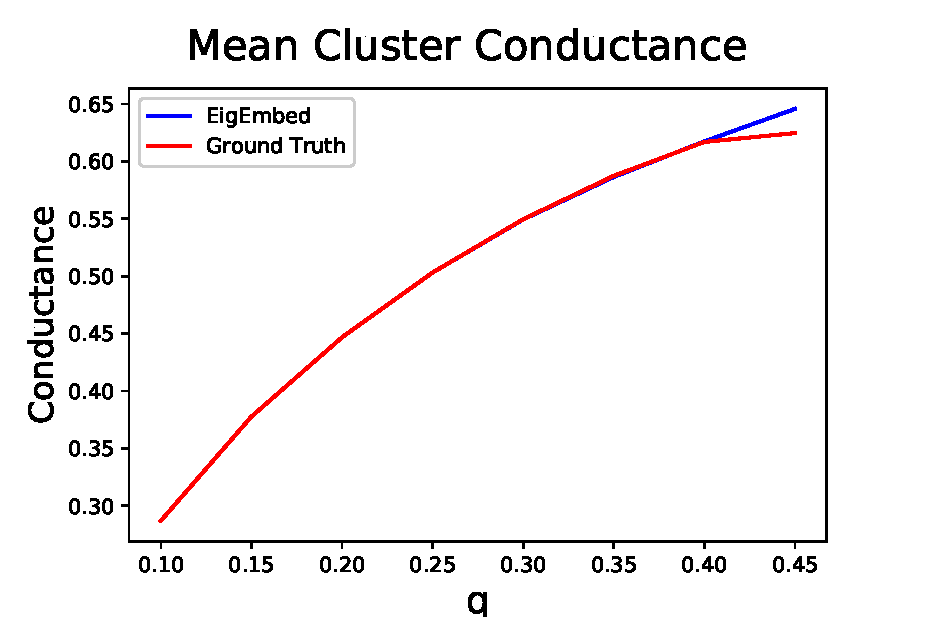
\includegraphics[width=.3\textwidth]{MCond_3b.eps}
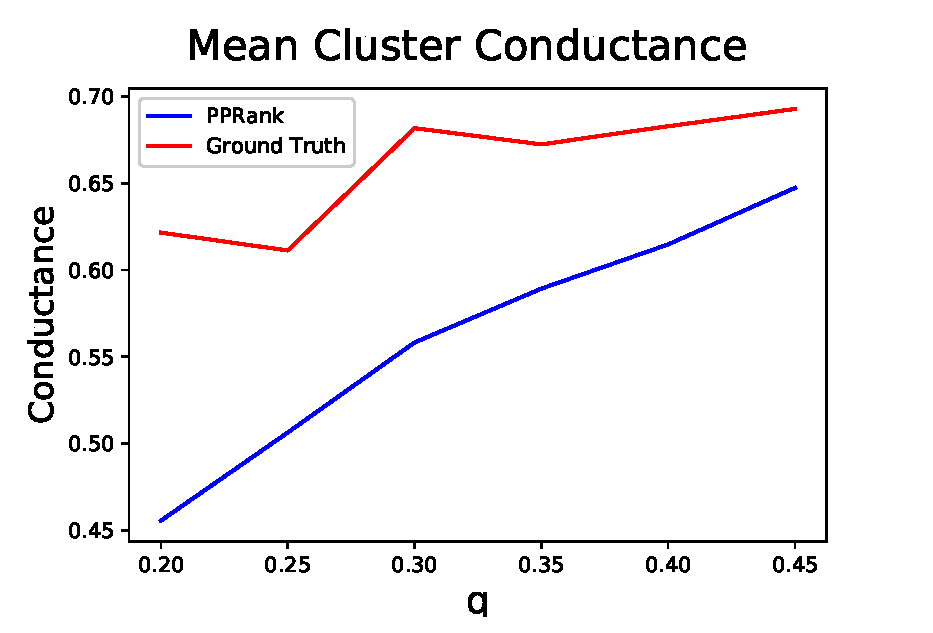
\includegraphics[width=.3\textwidth]{Cond_3b_pprank.eps}
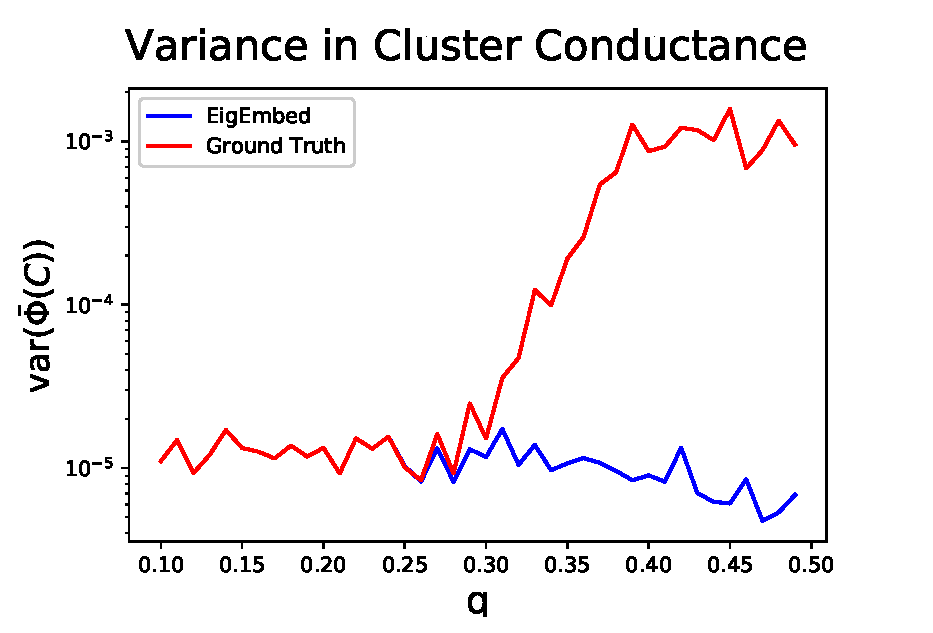
\includegraphics[width=.3\textwidth]{Cond_3b.eps}
%\includegraphics[width=.5\textwidth]{}
\caption{Mean conductance of computed clusters for \textbf{Left:} spectral clustering and \textbf{Middle:} local PageRank algorithms in the planted-partition model with three communities of 50 vertices. \textbf{Right:} Variance in conductance as an indicator of poor cluster quality.}\label{fig: Conductance}
\end{figure}

In Figure~\ref{fig: F1 Scores}, we compare the ability of spectral clustering and PageRank partitioning to recover the ground truth clusters. We measure this using the average F1 score of all clusters. The F1 score of a cluster is defined as
$$F_1 = 2 \cdot \frac{\text{precision}\cdot \text{recall}}{\text{precision}+\text{recall}},$$
where
$$\text{precision} = \frac{\#\text{true positive}}{\#\text{true positive + false positives}},$$
$$\text{recall} = \frac{\#\text{true positives}}{\#\text{true positives + false negatives}}.$$
To calculate the F1 score for a cluster, we first need to match a given recovered cluster to a ground truth cluster. We calculate the F1 score for each possible match and use the maximum score as the F1 score of the cluster.
\begin{figure}
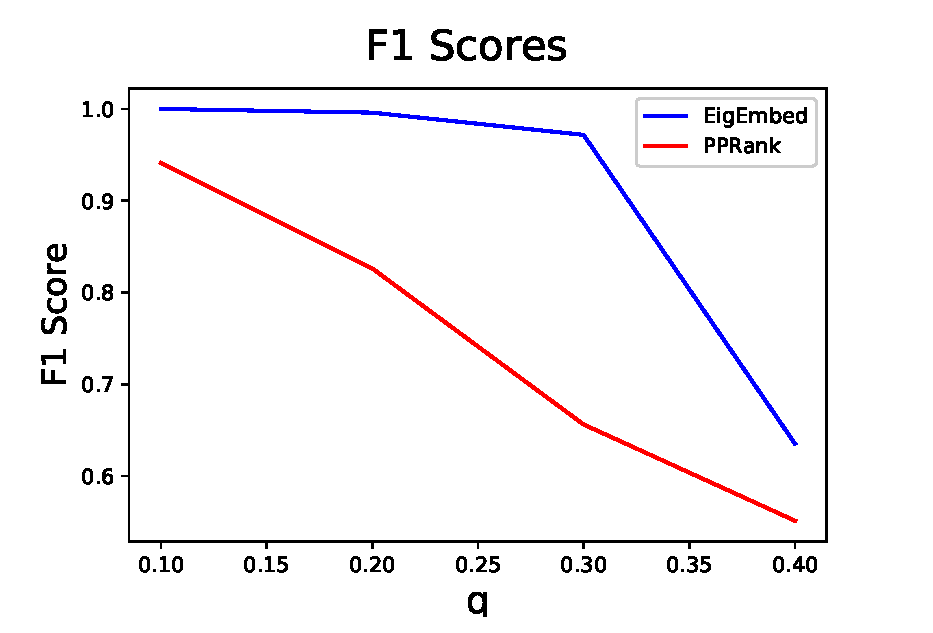
\includegraphics[width=.5\textwidth]{2b_p8_3.eps}
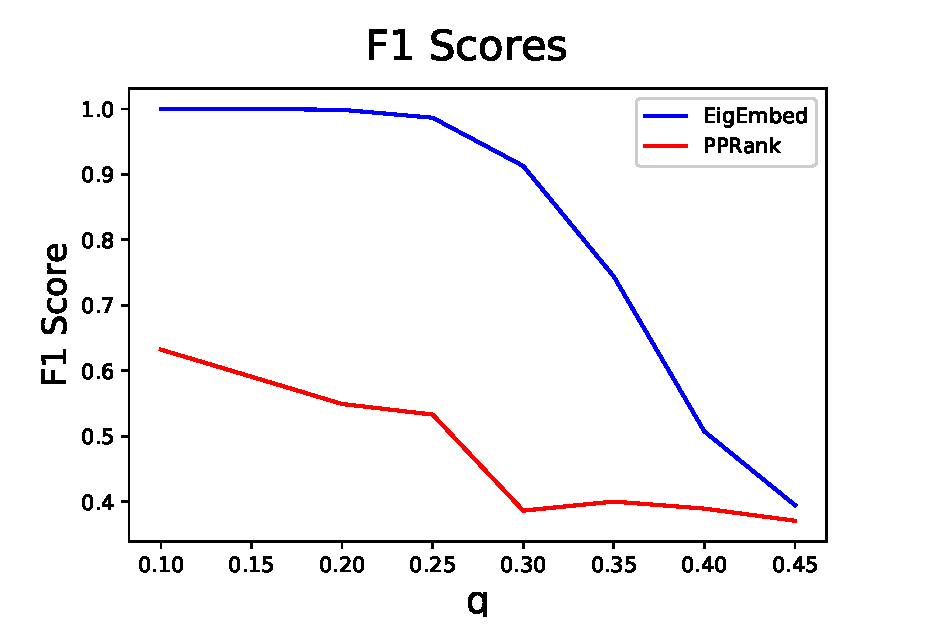
\includegraphics[width=.5\textwidth]{3b_p8_3.eps}
\caption{F1 scores achieved by spectral clustering and local PageRank for the planted-partition model with \textbf{Left:} two communities of 50 vertices and \textbf{Right:} three communities of 50 vertices.}\label{fig: F1 Scores}
\end{figure}

The experiments in Figures \ref{fig: Conductance} were performed on the planted partition model with three communities of $50$ nodes. This particular case was interesting because the spectral clustering algorithm (EigEmbed) accurately recovered the clusters up until $q\approx .35$ while the F1 score for the clusters recovered by the local clustering algorithm (PPRank) were quite low (See the right panel in Figure \ref{fig: F1 Scores}. However, the conductance plots in Figure \ref{fig: Conductance} show that PPRank recovered clusters with lower average conductance. In fact, while EigEmbed clusters the $150$ nodes into three balanced communities, PPRank consistently partitioned the $150$ nodes into two balanced communities and then subdivided one of these communities further, achieving a lower mean conductance than that of the `ground truth' clusters.

For the two block case (See the left panel of Figure \ref{fig: F1 Scores}), PPRank accurately recovers the clusters when the probability $q$ of edge connections between clusters is low, but the quality deteriorates rapidly as $q$ is increased. In both situations, spectral clustering maintains high quality recovery until $q\approx .35$.

Figure~\ref{fig:compute_time_pp} shows empirical time complexity on the planted partition model. Computation quickly became unwieldy for larger $k$ using PageRank clustering. This is expected, as the {\tt PageRank-Partition} time complexity depends on $m$, which is expected to scale with $n^2$ in planted partition. For spectral clustering we observe an approximately quadratic time complexity as the graph size ranges from $nk=100$ nodes to $nk=1000$ nodes. This is expected because the dominant cost of implicitly restarted Lanczos is the iterative application of matrix-vector products. Since the number of non-zeros $m$ scales with $n^2$ in the planted partition model with fixed $q$, the Laplacian becomes increasingly dense as $k$ increases. This assessment supports the observed quadratic complexity.

\begin{figure}
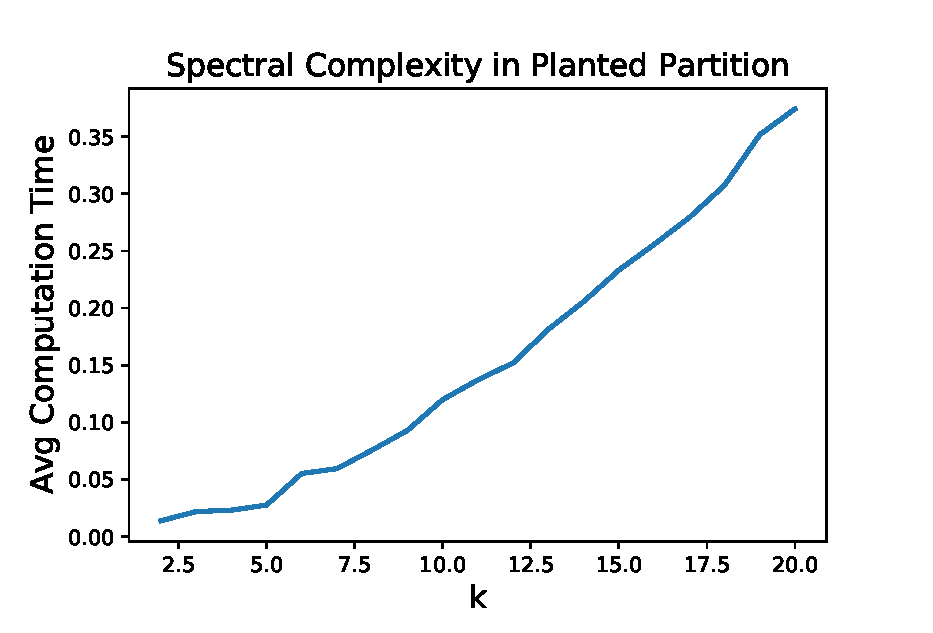
\includegraphics[width=.5\textwidth]{planted_partition_compute_time_spec.eps}
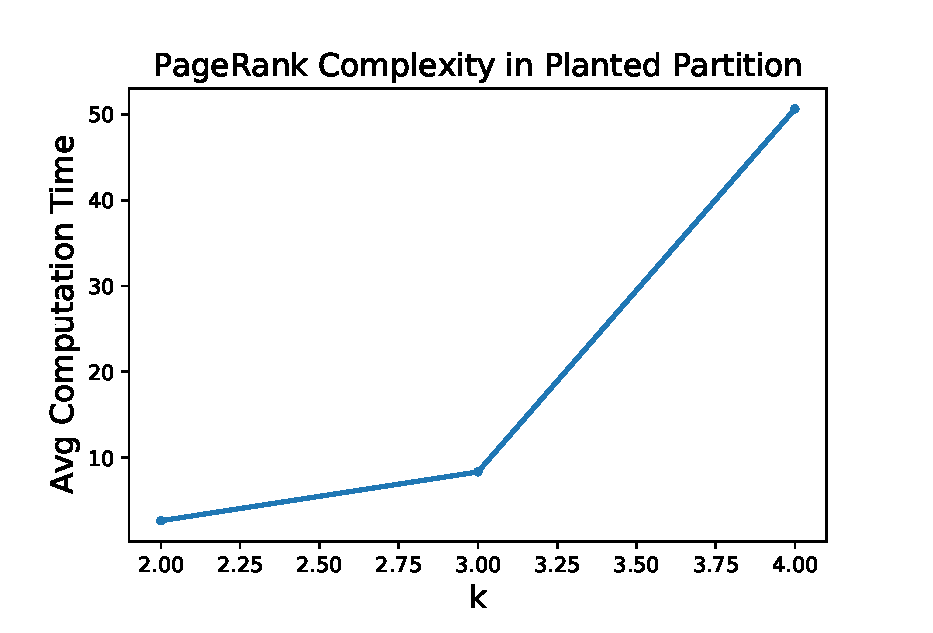
\includegraphics[width=.5\textwidth]{planted_partition_compute_time_pr.eps}
\caption{Average computation time over 20 trials to split planted partition graphs into two cluster. Parameter values: $n_1=50,p=0.5,q=0.2,\varphi=\max(0.5, 1.2\mu)$ and $k$ on the $x$-axis. \textbf{Left:} spectral clustering, \textbf{Right:} PageRank clustering (with {\tt PageRank-Partition} input $q=0.8$}\label{fig:compute_time_pp}
\end{figure}

Figure~\ref{fig:compute_time_sparse} shows empirical time complexity on sparse graphs generated from random trees. We consider sparse graphs since this should better reflect the strength of PageRank clustering. In this case, PageRank clustering is more competitive with spectral clustering but still increases faster as $n$ increases. This might be reduced with a more optimized implementation.
\begin{figure}
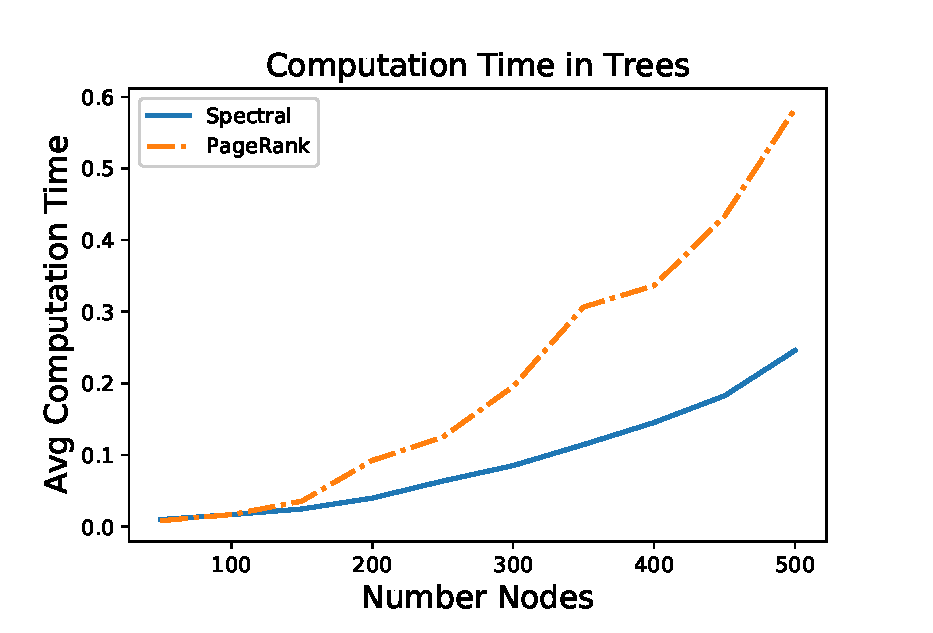
\includegraphics[width=.5\textwidth]{trees_compute_time.eps}
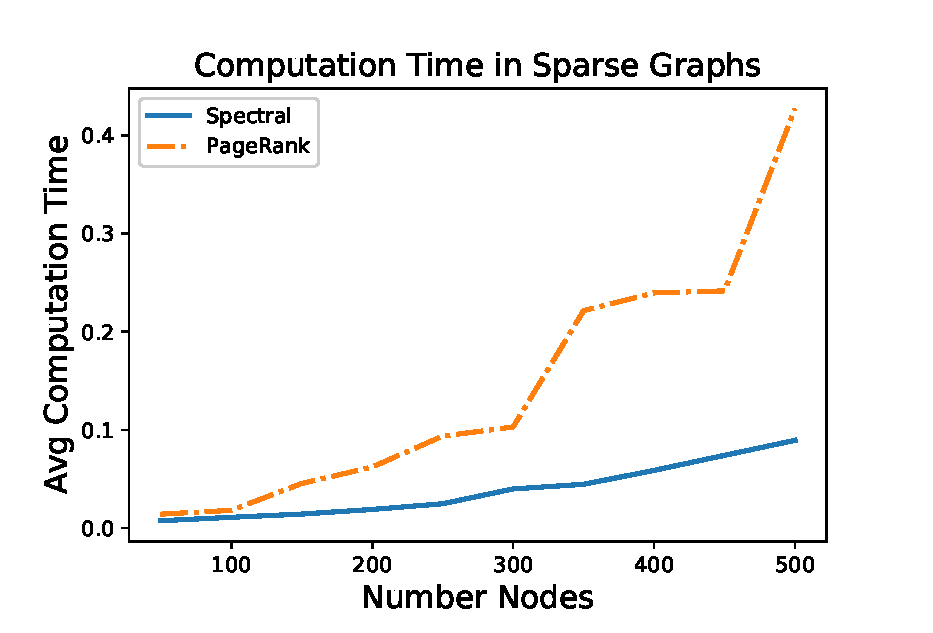
\includegraphics[width=.5\textwidth]{trees2_compute_time.eps}
\caption{Average computation time over 20 trials to split sparse graphs into two clusters. Sparse graphs generated using {\tt NetworkX} {\tt random\_powerlaw\_tree} with $\gamma = 3$. \textbf{Left:} single tree, \textbf{Right:} two tree edge sets added together. {\tt PageRank-Partition} implemented with $\varphi  =  0.5$, $q = 0.8$} \label{fig:compute_time_sparse}
\end{figure}







%%%%%%%%%%%%%%%%%%%%%%%%%%%%%%%%%%%%%%%%%%%%%
\section{A first application}
\label{Applications}

In this section, we apply our global and local clustering algorithms to a graph of one of the authors' Facebook friends circa 2014. These algorithms may be used to identify community structure and spheres of influence in a social network. Identifying these community structures may play a role in improved recommender and filtering systems \cite{}.

Our results are displayed in Figure \ref{fig:fb_graph}. With 6 clusters, neither EigEmbed or PPRank is perfect, but each algorithm picks up on interesting features. In particular, they both find low conductance sets, many of which correspond well with ground truth clusters. That said, PageRank clustering tended to break up some groups that perhaps shouldn't have been broken up. On the other hand, spectral clustering didn't break up such groups, but left some groups too large that should have been broken down (and ended up finding more smaller clusters). When using a higher number of clusters (e.g., 10 or more instead of 6), however, spectral clustering successfully breaks down these larger clusters.

\begin{figure}
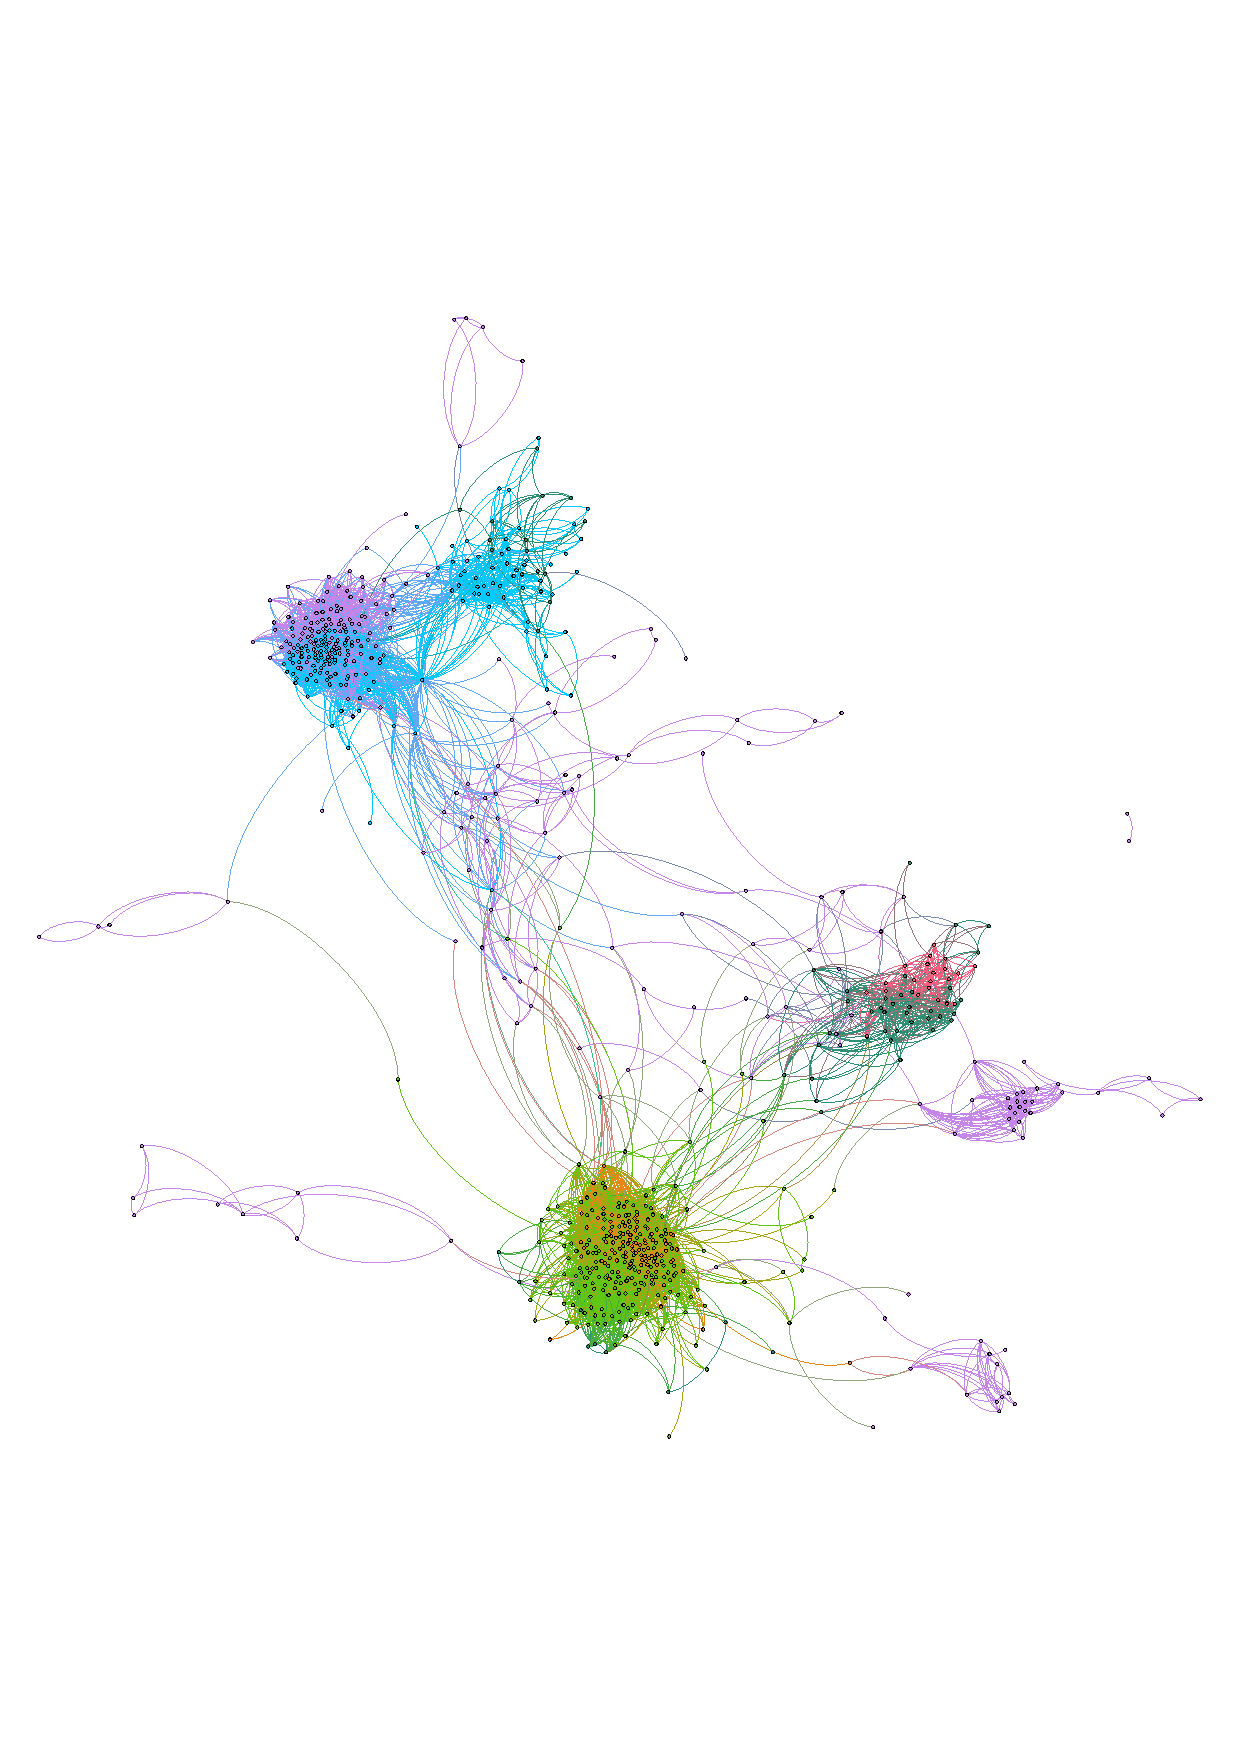
\includegraphics[width=.3\textwidth]{fb_graph_pr_cluster.pdf}
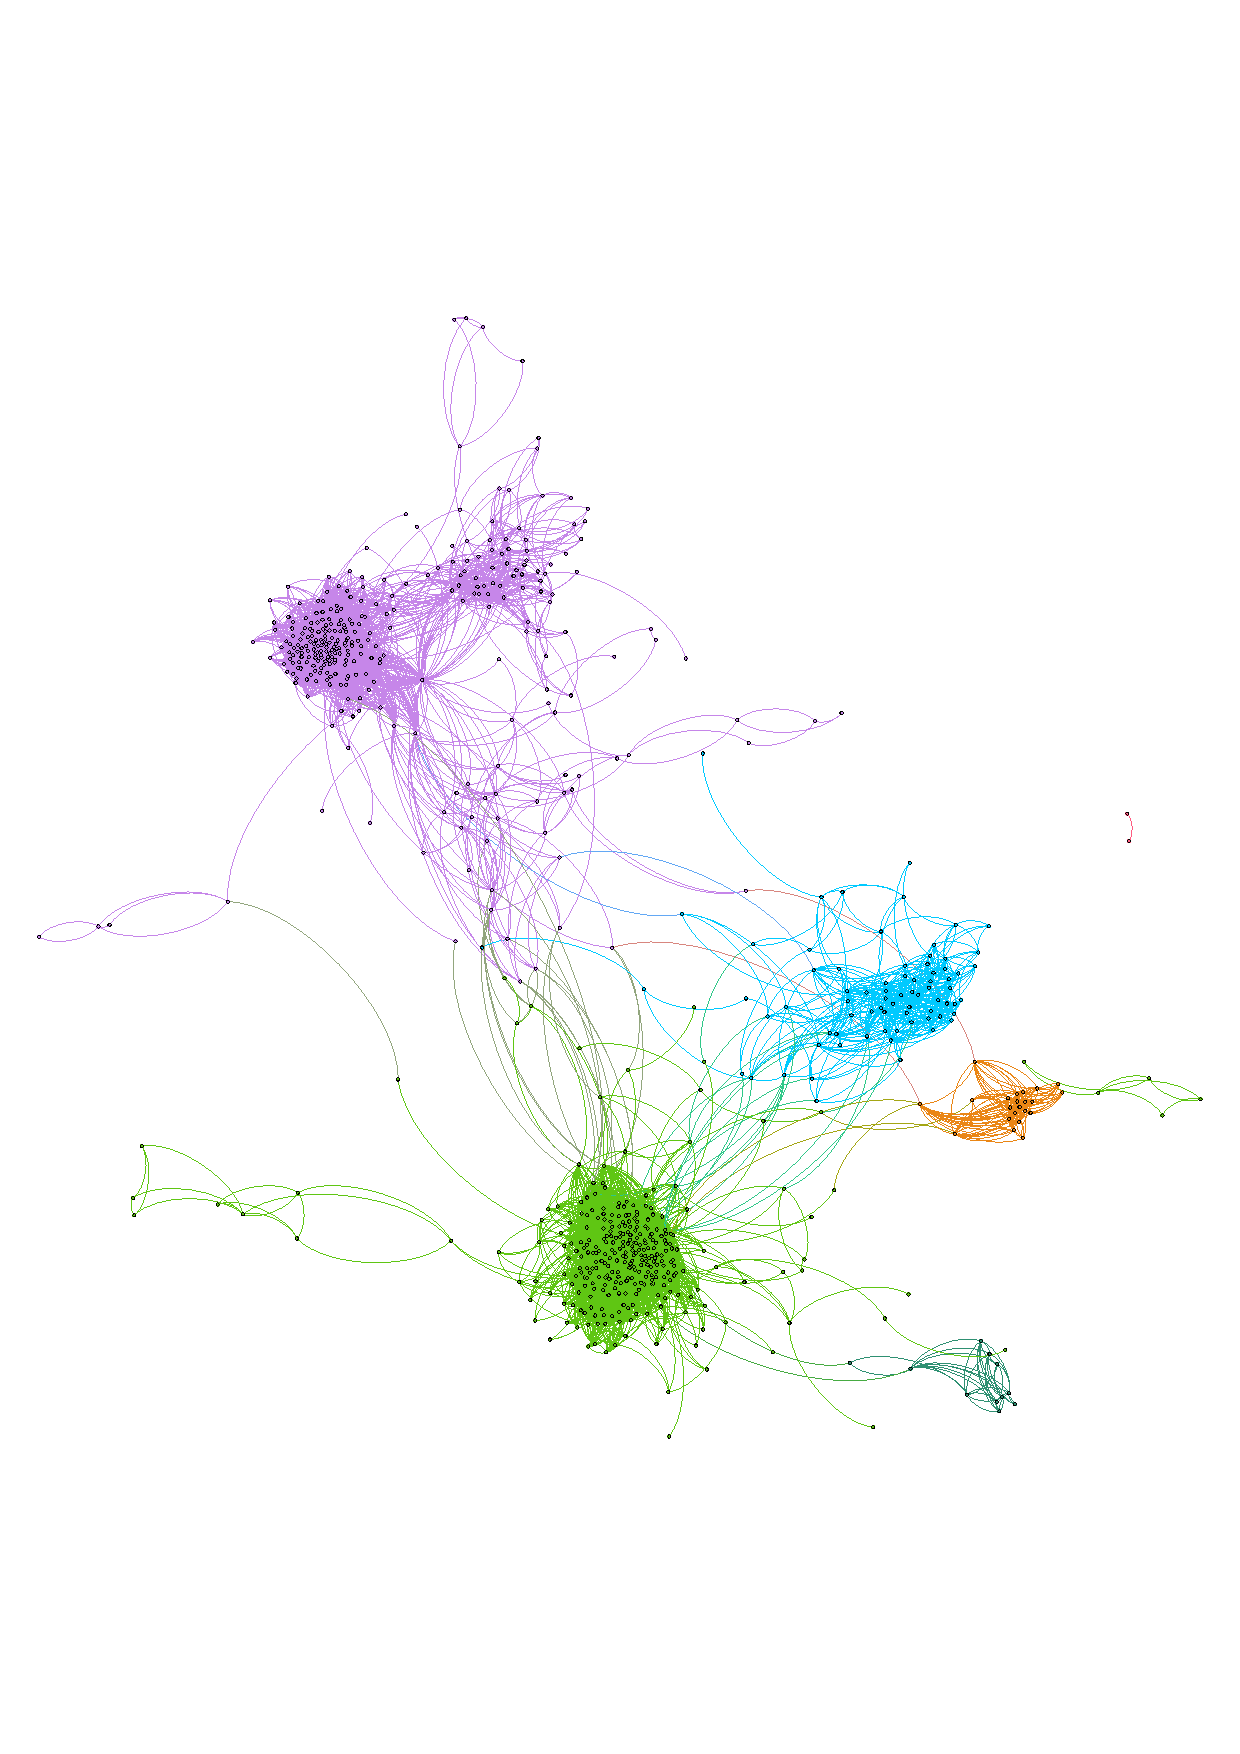
\includegraphics[width=.3\textwidth]{fb_graph_spec_cluster.pdf}
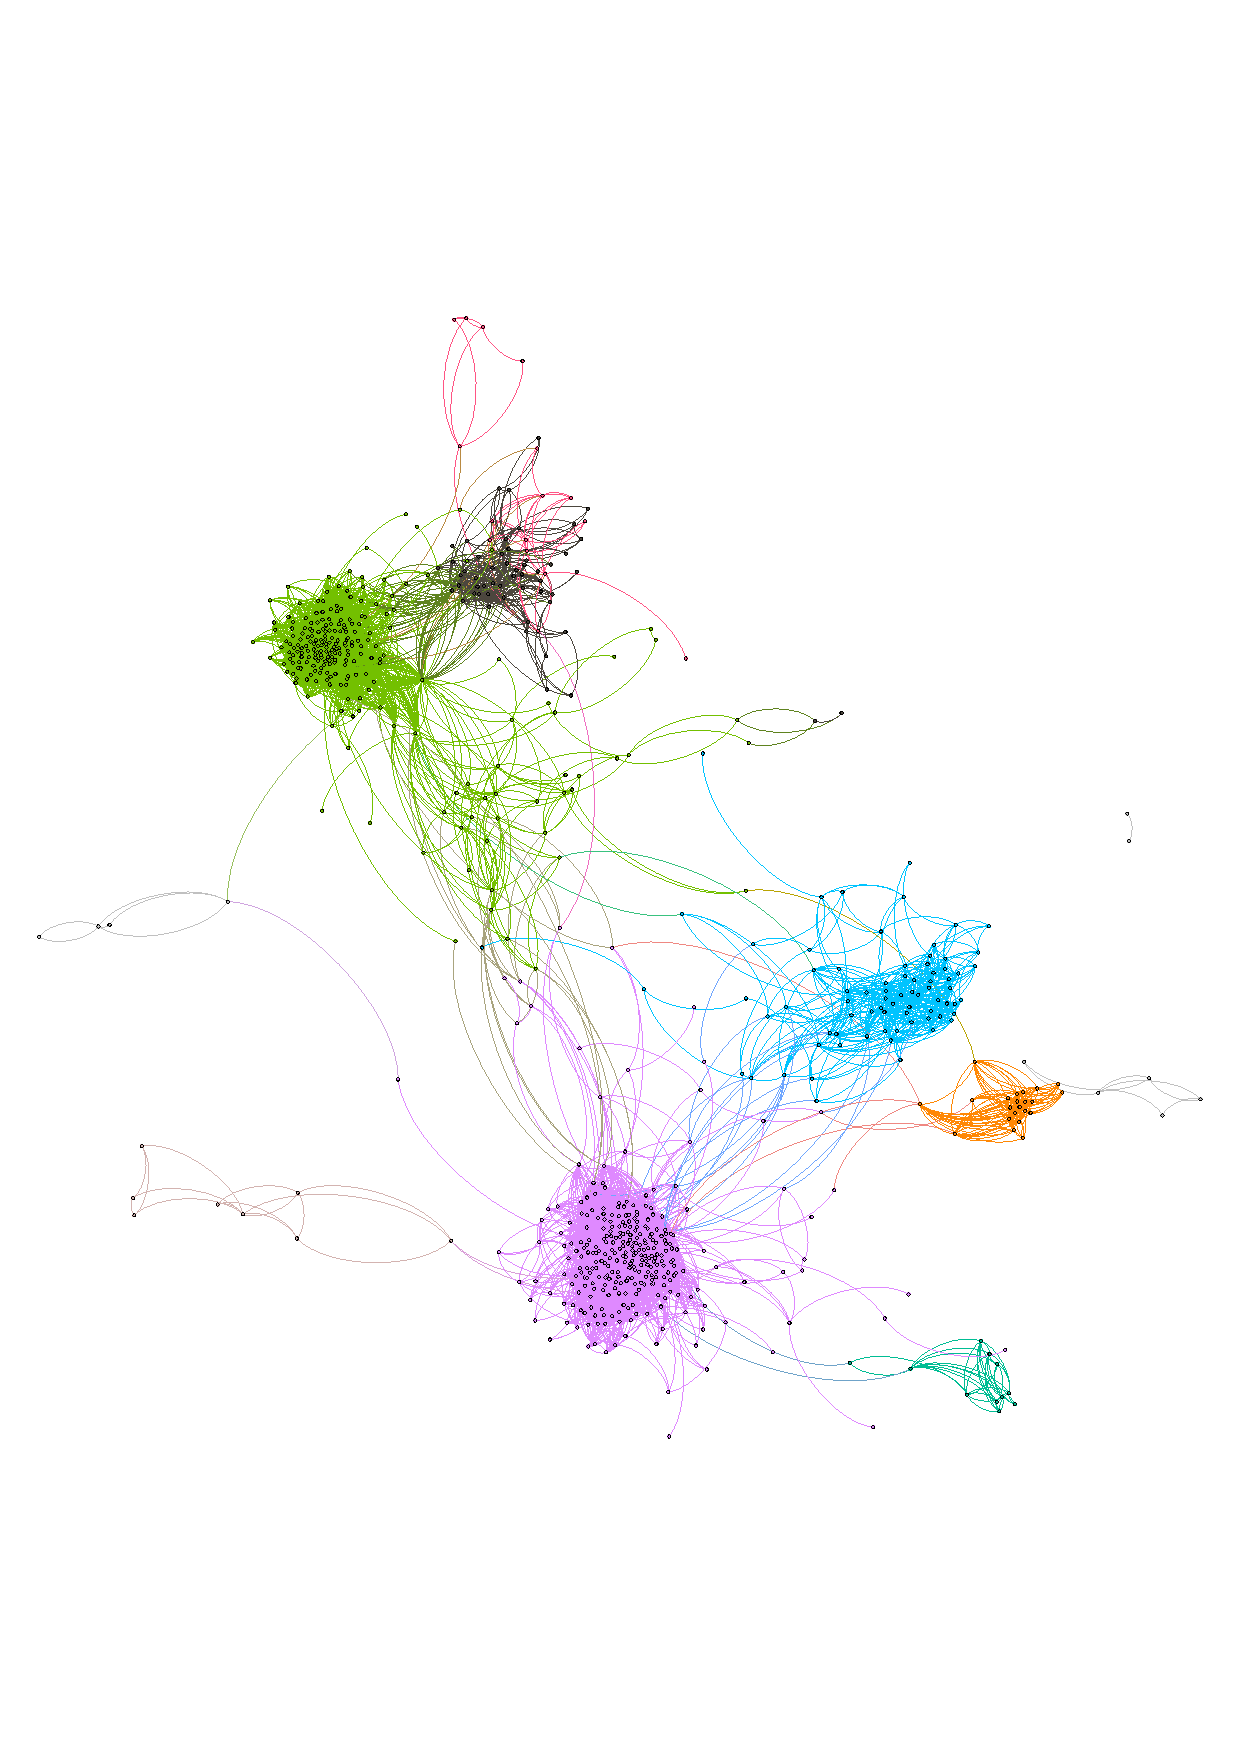
\includegraphics[width=.3\textwidth]{fb_graph_spec_cluster_10.pdf}
\caption{Facebook graph with \textbf{Left:} 6 PageRank clusters, \textbf{Middle:} 6 spectral clusters, \textbf{Right:} 10 spectral clusters.}\label{fig:fb_graph}
\end{figure}

%%%%%%%%%%%%%%%%%%%%%%%%%%%%%%%%%%%%%%%%%%%%%
\section{Discussion}
\label{Discussion}

In this report, we have presented the relevant theoretical and algorithmic ideas associated with a global graph clustering technique based on an eigenvector embedding and a local graph clustering based on local stochastic exploration of the graph. We have developed implementations of both methods and tested their performance on well-studied generative cluster models. Finally, we applied both algorithms to a real-world graph representing an online social network.

We now discuss some observations from using these methods.
\begin{itemize}
\item First, we note that {\tt PageRank-Partition} is easy to parallelize. Eigenvector calculations, on the other hand, are notoriously difficult to parallelize. While some eigensolvers based on spectral projection, such as FEAST, are highly parallelizable, these typically require some localization of the desired eigenvalues in the complex plane \cite{FEAST}. This information may be difficult unless some detailed spectral properties (such as spectral gap information) of the graph are known.

\item For three clusters in the planted partition model, PageRank clustering tends to produce one cluster containing half the nodes and two clusters each containing one quarter of the nodes. This is using $p=0.5,q=0.2$ and a range of $\varphi$ values around 0.5 (the expected conductance of the clusters is around $0.44$). This might help to explain why higher order methods (e.g., considering triangles in the graph) might recover more information about the planted partitions, as indicated in \cite{benson}. The idea is that the difference in edge probabilities might be small, but the triangle probabilities will still be more distinct, at least in the planted partition model.

\item A major difficulty in using PageRank clustering is choosing a value of the threshold $\varphi$. Choosing too low a value tends to make the PageRank method run too long (even if there is a set with conductance less than $\varphi$), whereas choosing a value of $\varphi$ too high yields poor partitioning. This is expected, however, as the time complexity depends on $1/\varphi^3$.

\item Related to the above point, the theoretical guarantee for PageRank clustering seems weak. In particular, for the planted partition model, it only seems to apply when there is a very large distinction between $p$ and $q$. This is because the theorem requires a cut with conductance so much smaller than $\varphi$ to ensure finding a cut with conductance less than $\varphi$. If the minimum conductance in the graph is not very low, the corresponding value of $\varphi$ may be greater than 1, and so not useful. Because of this, the theoretical guarantee doesn't seem to be useful on a practical front.

\end{itemize}










%%%%%%%%%%%%%%%%%%%%%%%%%%%%%%%%%%%%%%%%%%%%%%%%%%%%%%%%%%%%%%%%%%%%%%%%%%%%%%%%%%%%%%%%%



\begin{thebibliography}{10}

\bibitem{pagerank_cluster}
	R. Andersen, F. Chung, and K. Lang,
	\emph{Local graph partitioning using pagerank vectors},
	In FOCS, 2006,
	available at \url{http://ieeexplore.ieee.org/document/4031383/}.

\bibitem{benson}
	H. Yin, A. Benson, J. Leskovec, D. Gleich,
	\emph{Local higher-order graph clustering},
	In KDD, 2017,
	available at \url{https://cs.stanford.edu/people/jure/pubs/mappr-kdd17.pdf}.

\bibitem{spielman}
	D. Spielman, S. Teng,
	\emph{Nearly-linear time algorithms for graph partitioning, graph sparsification, and solving linear systems},
	In ACM STOC-04, pages 81?90, New York, NY, USA, 2004. ACM Press.
	available at \url{https://arxiv.org/abs/cs/0310051}.
    
\bibitem{luxburg}
	Ulrike von Luxburg, 
    \emph{A Tutorial on spectral clustering}, 
    2007,
    available at \url{http://citeseerx.ist.psu.edu/viewdoc/summary?doi=10.1.1.165.9323}.

\bibitem{shi}
	J. Shi, and J. Malik,
	\emph{Normalized cuts and image segmentation},
	In TPAMI, Volume: 22, Issue: 8, pages 888?905 Aug 2000. IEEE.
	available at \url{http://ieeexplore.ieee.org/document/868688/}.
    
\bibitem{recommenders}
	X. Li, Z. Wang, R. Hu, et al.,
    \emph{Recommendation algorithm based on improved spectral clustering and transfer learning},
    In PAA, 2017,
    available at \url{https://doi.org/10.1007/s10044-017-0671-2}.

\bibitem{spielman_clustering_works}
	D. Spielman and S. Teng,
    \emph{Spectral partitioning works: Planar graphs and
finite element meshes},
	in IEEE Symposium on Foundations of Computer Science, pages 96–
105, 1996,
	available at \url{http://www.cs.cornell.edu/courses/cs6822/2011fa/papers/ST_spectral_works.pdf}.

\bibitem{high_dim_data}
	S. Wu, X. Feng, W. Zhou,
    \emph{Spectral clustering of high-dimensional data exploiting sparse representation vectors},
    In Neurocomputing, Volume 135, 2014, Pages 229-239, ISSN 0925-2312, 		available at \url{https://doi.org/10.1016/j.neucom.2013.12.027}.

\bibitem{social_network}
    Ulzii-Utas Narantsatsralt and Sanggil Kang,
    \emph{Social Network Community Detection Using Agglomerative Spectral Clustering}, 
    In Complexity, vol. 2017, Article ID 3719428, 10 pages, 2017. 
    available at \url{https://doi.org/10.1155/2017/3719428}.

\bibitem{FEAST}
	E. Polizzi, 
	\emph{Density-Matrix-Based Algorithms for Solving Eigenvalue Problems}, 
	In Phys. Rev. B. Vol. 79, 115112 (2009),
    available at \url{https://arxiv.org/pdf/0901.2665.pdf}.


\end{thebibliography}








\end{document}
